\documentclass[11pt, pdftex]{article}
\usepackage[margin=1in]{geometry}
\usepackage{graphicx}
\usepackage{amsmath}
\usepackage{listings}
\usepackage{semantic}
\usepackage[hyphens]{url}
\usepackage[breaklinks]{hyperref}
\usepackage[demo]{graphicx}
\usepackage{subcaption}
\usepackage{hyperref}
\title{Assignment (MiniProject) #1}
\author{Machiry Aravind Kumar}
\date{UCSB}
\begin{document}
\maketitle
\section{Datasets}
I selected 2 datasets for this homework.
\begin{itemize}
\item Mammographic Mass Data Set\\
This dataset is from UCI Archive: \url{https://archive.ics.uci.edu/ml/datasets/Mammographic+Mass}. Mammography is the most effective method for breast cancer screening available today. The provided dataset has 961 samples, with 5-features and a classification of benign(0) or malignant(1). Features in the dataset are:
\begin{itemize}
\item BI-RADS assessment: 1 to 5 (ordinal, non-predictive!)
\item Age: patient's age in years (integer)
\item Shape: mass shape: round=1 oval=2 lobular=3 irregular=4 (nominal)
\item Margin: mass margin: circumscribed=1 microlobulated=2 obscured=3 ill-defined=4 spiculated=5 (nominal)
\item Density: mass density high=1 iso=2 low=3 fat-containing=4 (ordinal) 
\item Severity: benign=0 or malignant=1 (binominal, target class) 
\end{itemize}
Based on the distribution of features as shown in Figure \ref{fig:mam}.
\item Wine Dataset \\
Again, this dataset is from UCI archive: \url{http://archive.ics.uci.edu/ml/datasets/Wine}. This data are the results of a chemical analysis of wines grown in the same region in Italy but derived from three different cultivars. The analysis determined the quantities of 13 constituents found in each of the three types of wines. Thus dataset has 13 features and for this homework I used Feature 13 (Proline value) and corresponding distribution is as shown in Figure \ref{fig:wine}. Also, This dataset has 3 classes (3 types of wines) but because of the restriction, I selected data for only 2 classes (i.e 2 types of wines: 1 and 2)
\end{itemize}

\begin{figure}
\begin{subfigure}
  \centering
  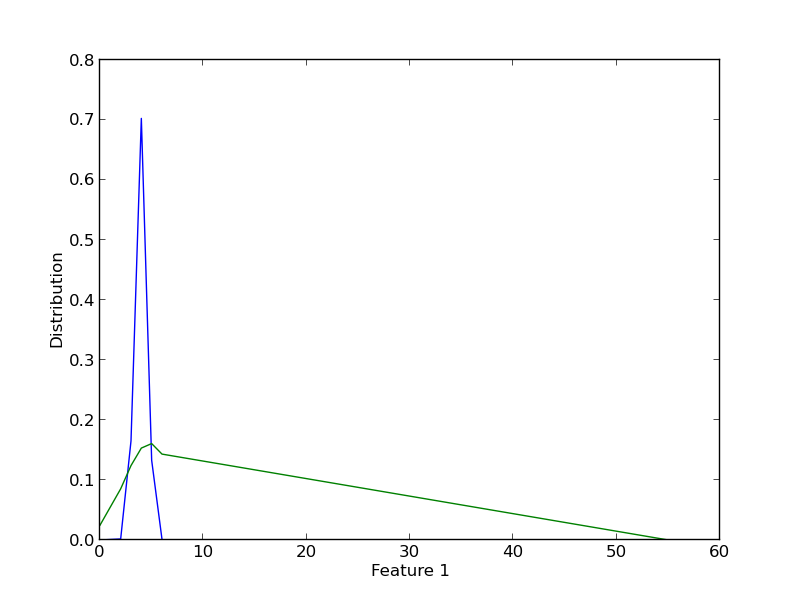
\includegraphics[width=0.5\textwidth]{pics/mam1.png}
\end{subfigure}
\begin{subfigure}
  \centering
  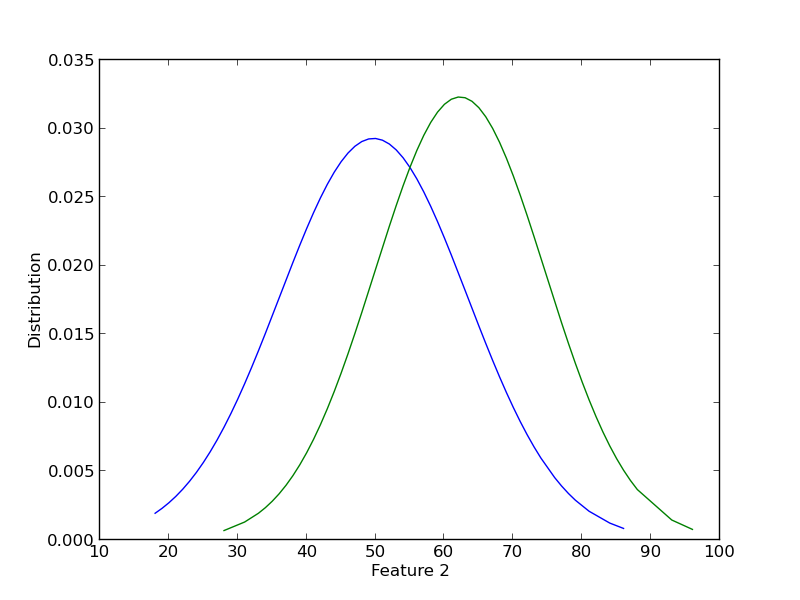
\includegraphics[width=0.5\textwidth]{pics/mam2.png}
\end{subfigure}
\begin{subfigure}
  \centering
  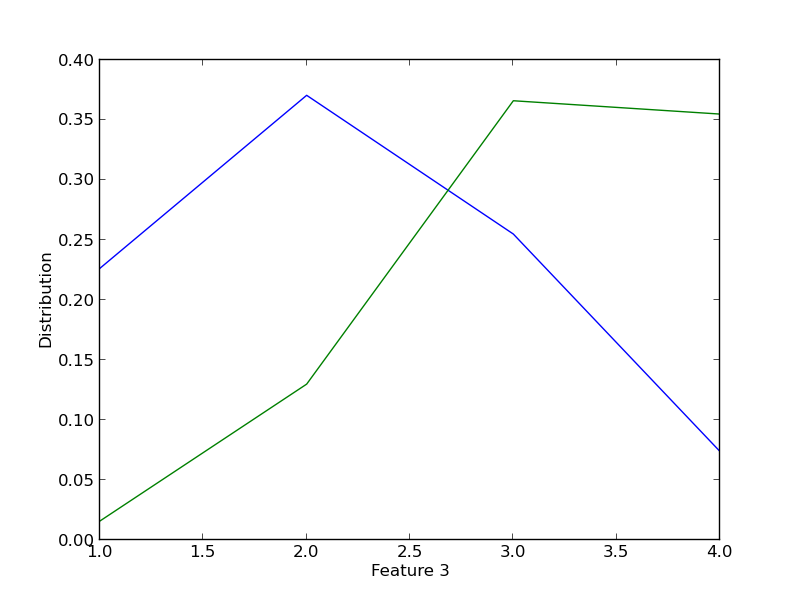
\includegraphics[width=0.5\textwidth]{pics/mam3.png}
\end{subfigure}
\begin{subfigure}
  \centering
  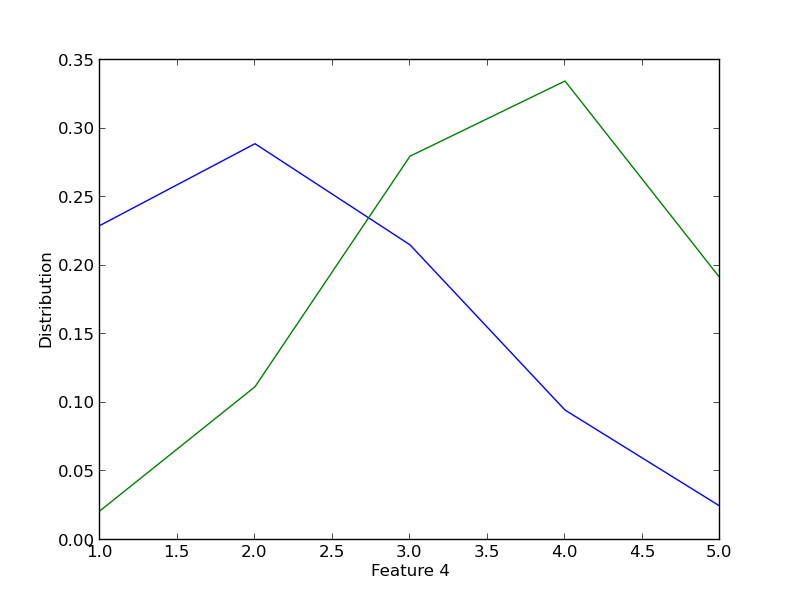
\includegraphics[width=0.5\textwidth]{pics/mam4.png}
\end{subfigure}
\begin{subfigure}
  \centering
  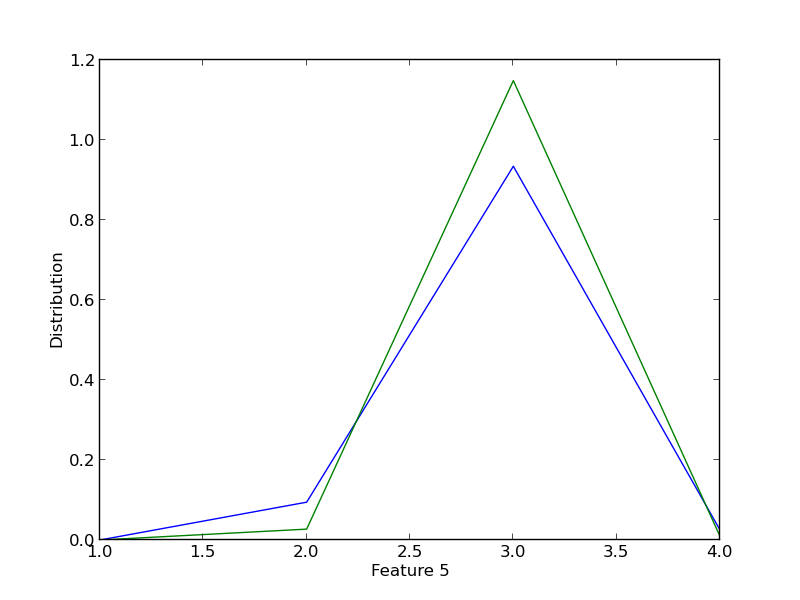
\includegraphics[width=0.5\textwidth]{pics/mam5.png}
\end{subfigure}
\caption{Mammographic features distribution}
\label{fig:mam}
\end{figure}

\begin{figure}
    \centering
    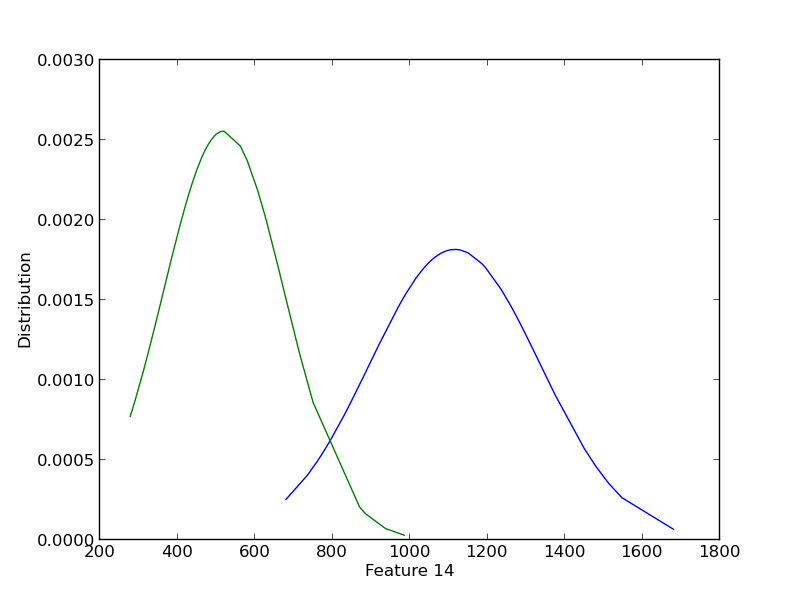
\includegraphics[width=0.6\textwidth]{pics/wine14.png} 
    \caption{Feature Proline distribution}
    \label{fig:wine}
\end{figure}
\section{Parametric Values for the Datasets}
\subsection{Mammographic dataset}
Mean For 2 classes :49.71317829, 62.25909091. \\
Standard deviation:185.59215191, 152.4828719. \\
The graph is same as the graph for Feature 2 in Figure \ref{fig:mam}.
\subsection{Wine dataset}
Mean:1115.71186441, 519.50704225. \\
Standard deviation: 48239.7305372, 24367.26403491.
The graph is same as the one in Figure \ref{fig:wine}.
\section{Computing best dichotomy parameters}
I used a modified binary search to find the right value for dichotomy, the code for which is present at: $\texttt{parametric\_est.py}$. Values for the 2 datasets is as shown below:
\subsection{Mammographic dataset}
Best feature Dichotomy value: 58.25.\\
\subsection{Wine dataset}
Best feature Dichotomy value: 980.37109375.\\
\section{Classification Accuracy}
The accuracy for different values of n for n-fold validation on different datasets is shown below:
\subsection{Wine dataset}
The results for different values of n are as shown in Table \ref{tab:wine}
\begin{table}
\centering
\begin{tabular}{ | c | c |}
    \hline
    {\bf N} & {\bf Mean Accuracy} \\ 
    \hline
    3 & 0.923\\
	\hline
	4 & 0.931\\
	\hline
	5 & 0.923\\
	\hline
	6 & 0.922\\
	\hline
	7 & 0.923\\
	\hline
	8 & 0.923\\
	\hline
	9 & 0.923\\
	\hline
	10 & 0.923\\
	\hline
	\end{tabular}
	\caption{Cross Validation Results for Wine}
    \label{tab:wine}
\end{table}
\subsection{Mammographic dataset}
The results for different values of n are as shown in Table \ref{tab:man}
\begin{table}
\centering
\begin{tabular}{ | c | c |}
    \hline
    {\bf N} & {\bf Mean Accuracy} \\ 
    \hline
    3 & 0.672\\
	\hline
	4 & 0.678\\
	\hline
	5 & 0.671\\
	\hline
	6 & 0.678\\
	\hline
	7 & 0.677\\
	\hline
	8 & 0.678\\
	\hline
	9 & 0.676\\
	\hline
	10 & 0.676\\
	\hline
	\end{tabular}
	\caption{Cross Validation Results for Mammographic}
    \label{tab:man}
\end{table}
\end{document}